\lstset{
  basicstyle=\ttfamily,
  columns=fullflexible,
  frame=single,
  breaklines=true,
  postbreak=\mbox{\textcolor{red}{$\hookrightarrow$}\space},
}
\chapter{Implementasi dan Pengujian}
\label{chap:implementasiDanPengujian}
\setcounter{secnumdepth}{3}
\paragraph{}Setelah dilakukan perancangan dan analisis sistem kini dan sistem usulan, maka langkah berikutnya adalah mengimplementasikannya ke dalam sistem baru.
\section{Implementasi}
Pada bagian ini akan dijelaskan secara rinci implementasi perancangan-perancangan pada Bab 3 ke dalam sistem.
\subsection{Lingkungan Pengembangan dan Pengujian Fungsional}
\paragraph{} Pembangunan perangkat lunak ini memakai bahasa pemrogaraman server PHP 5 dan MySQL 5.0 sebagai basis datanya. Pengembangan perangkat lunak ini dilakukan di komputer dengan spesifikasi perangkat keras dan perangkat lunaknya sebagai berikut:
\begin{itemize}
\item \textbf{Perangkat Keras}
\begin{enumerate}
	\item Prosesor AMD A6 VISION
	\item RAM 4 GB
	\item 500 GB harddisk
	\item Monitor
	\item Keyboard
	\item Mouse
\end{enumerate}
\item \textbf{Perangkat Lunak}
\begin{enumerate}
	\item Sistem Operasi Windows 8
	\item NetBeans IDE 8.0.2
	\item Server phpMyAdmin 4.3.11
	\item XAMPP Control Panel v3.2.1
	\item Client: Google Chrome 61.0.3163.100 32-bit
	\item Microsoft Excel 2013
\end{enumerate}

\end{itemize}
\subsection{Implementasi Basis Data}
\paragraph{}Implementasi basis data dalam Aplikasi Pembangkit Jadwal Dosen menggunakan satu tabel basis data. Tabel tersebut adalah tabel jadwal\_dosen yang menyimpan informasi-informasi seperti:
\begin{enumerate}
	\item user yang memiliki jadwal terkait
	\item hari berlangsungnya jadwal
	\item jam dimulainya kegiatan jadwal 
	\item durasi (dalam jam) lama berlangsungya jadwal
	\item nama kegiatan jadwal
	\item waktu terakhir jadwal diupdate
\end{enumerate}

\subsection{Implementasi Kelas}
Implementasi kelas dalam Aplikasi Pembangkit Jadwal Dosen terdiri dari kelas - kelas sebagai berikut:
\begin{enumerate}
	\item Kelas \textit{controller} EntriJadwalDosen\\
	Merupakan kelas yang mengatur hubungan antara kelas view EntriJadwalDosen dan kelas model JadwalDosen\_model.
	\item Kelas \textit{controller} LihatJadwalDosen\\
	Merupakan kelas yang berfungsi menghubungkan antara kelas view LihatJadwalDosen dan kelas model JadwalDosen\_model.
	\item Kelas \textit{view} EntriJadwalDosen yang berfungsi membuat \textit{user interface} untuk memasukan jadwal dan menampilkan jadwal milik pengguna itu sendiri.
	\item Kelas \textit{view} LihatJadwalDosen yang berfungsi membuat \textit{user interface} untuk melihat jadwal dan menmpilkan opsi untuk ekspor jadwal ke XLS.
	\item Kelas model JadwalDosen\_model yang berfungsi untuk menulis atau membaca ke basis data.
	\item Kelas \textit{config} modules yang berfungsi untuk membatasi hak ases pengguna.
\end{enumerate}

\section{Pengujian}
\paragraph{} Pengujian aplikasi ini dilakukan dengan menggunakan metode pengujian \textit{Black-Box Testing}. Pengujian ini difokuskan pada pengujian fungsional. Maksud dari pengujian fungsional ini adalah untuk menguji reaksi perangkat lunak terhadap aksi yang dilakukan oleh pengguna. Bila reaksi sistem tidak sesuai yang diharapkan, maka aplikasi masih memilki kekurangan.

\subsection{Hasil Pengujian}
Pada bagian ini akan dijelaskan mengenai hasil pengujian-pengujian sistem.
\subsubsection{Hasil Pengujian Login}
Hasil pengujian dapat dilihat pada Tabel 5.1
\begin{center}
	\begin{table}[H]
		\caption{Pengujian Login}
		\begin{tabular}{|p{5cm}|p{5cm}|p{5cm}|}
		\hline
		\centering Aksi	& 	\centering Reaksi yang diharapkan &  \multicolumn{1}{c|}{Reaksi PL} \\
		\hline
		Menekan tombol login & Menampilkan menu login & Menampilkan menu login \\
		\hline
		\end{tabular}
	\end{table}
\end{center}

\subsubsection{Hasil Pengujian Memasukkan Jadwal}
Hasil pengujian dapat dilihat pada Tabel 5.2
\begin{center}
	\begin{table}[H]
		\caption{Pengujian Memasukkan Jadwal}
		\begin{tabular}{|p{5cm}|p{5cm}|p{5cm}|}
		\hline
		\centering Aksi	& 	\centering Reaksi yang diharapkan &  \multicolumn{1}{c|}{Reaksi PL} \\
		\hline
		Memasukan data yang diperlukan untuk input jadwal & Jadwal yang sudah dimasukan muncul pada halaman Entri Jadwal Dosen & Jadwal yang sudah dimasukan muncul pada halaman Entri Jadwal Dosen \\
		\hline
		Data jadwal yang dimasukan tidak lengkap & Jadwal dimasukan dengan data yang sesuai nilai \textit{default} yang ditampilkan di menu & Jadwal dimasukan dengan data yang sesuai nilai \textit{default} yang ditampilkan di menu \\
		\hline
		Waktu dimulainya jadwal baru sama dengan jadwal yang sudah pernah dimasukan sebelumnya & Menampilkan pesan kesalahan dan batal memasukan data ke dalam database & Jadwal masuk ke dalam database, namun tidak muncul di halaman Entri Jadwal Dosen maupun halaman Lihat Jadwal Dosen \\
		\hline
		\end{tabular}
	\end{table}
\end{center}

\subsubsection{Hasil Pengujian Pengubahan Jadwal}
Hasil pengujian dapat dilihat pada Tabel 5.3
\begin{center}
	\begin{table}[H]
		\caption{Pengujian Pengubahan Jadwal}
		\begin{tabular}{|p{5cm}|p{5cm}|p{5cm}|}
		\hline
		\centering Aksi	& 	\centering Reaksi yang diharapkan &  \multicolumn{1}{c|}{Reaksi PL} \\
		\hline
		Memilih jadwal yang akan diedit & Memunculkan modal yang berisi menu edit yang menampilkan data jadwal yang sedang dipilih tersebut. Data tersebut juga dapat diubah oleh pengguna sesuai kebutuhannya & Memunculkan modal yang berisi menu edit yang menampilkan data jadwal yang sedang dipilih tersebut. Data tersebut juga dapat diubah oleh pengguna sesuai kebutuhannya \\
		\hline
		Memilih tombol simpan & Modal ditutup , data jadwal di \textit{database} diupdate sesuai dengan input user dan menampilkan menu Entri Jadwal Dosen & Modal ditutup , data jadwal di \textit{database} diupdate sesuai dengan input user dan menampilkan menu Entri Jadwal \\
		\hline
		Memilih tombol keluar & Modal ditutup lalu menampilkan menu Entri Jadwal Dosen & Modal ditutup lalu menampilkan menu Entri Jadwal Dosen \\
		\hline
		\end{tabular}
	\end{table}
\end{center}

\subsubsection{Pengujian Fungsional Hapus Jadwal Dosen}
Hasil pengujian dapat dilihat pada Tabel 5.4
\begin{center}
	\begin{table}[H]
		\caption{Pengujian Fungsional Hapus Jadwal Dosen}
		\begin{tabular}{|p{5cm}|p{5cm}|p{5cm}|}
		\hline
		\centering Aksi	& 	\centering Reaksi yang diharapkan &  \multicolumn{1}{c|}{Reaksi PL} \\
		\hline
		Memilih jadwal yang akan diedit & Memunculkan modal yang berisi menu edit yang menampilkan data jadwal yang sedang dipilih tersebut. Data tersebut juga dapat diubah oleh pengguna sesuai kebutuhannya & Memunculkan modal yang berisi menu edit yang menampilkan data jadwal yang sedang dipilih tersebut. Data tersebut juga dapat diubah oleh pengguna sesuai kebutuhannya \\
		\hline
		Memilih tombol hapus & Modal ditutup dan jadwal dihapus dari basis data, lalu sistem menampilkan menu Entri Jadwal Dosen & Modal ditutup dan jadwal dihapus dari basis data, lalu sistem menampilkan menu Entri Jadwal Dosen \\
		\hline
		Memilih tombol keluar & Modal ditutup lalu menampilkan menu Entri Jadwal Dosen & Modal ditutup lalu menampilkan menu Entri Jadwal Dosen \\
		\hline
		\end{tabular}
	\end{table}
\end{center}

\subsubsection{Hasil Pengujian Melihat Jadwal Dosen}
Hasil pengujian dapat dilihat pada Tabel 5.5
\begin{center}
	\begin{table}[H]
		\caption{Pengujian Melihat Jadwal Dosen}
		\begin{tabular}{|p{5cm}|p{5cm}|p{5cm}|}
		\hline
		\centering Aksi	& 	\centering Reaksi yang diharapkan &  \multicolumn{1}{c|}{Reaksi PL} \\
		\hline
		Menekan tombol Lihat Jadwal Dosen & 
		Sistem menampilkan semua jadwal dosen dan mengelompokannya ke dalam tab-tab berdasarkan email setiap pemilik jadwal terkait. Kemudian setiap tab diberi label berisi nama lengkap pemilik jadwal tersebut. &
		Sistem menampilkan semua jadwal dosen dan mengelompokannya ke dalam tab-tab berdasarkan email setiap pemilik jadwal terkait. Kemudian setiap tab diberi label berisi nama lengkap pemilik jadwal tersebut.\\
		\hline
		\end{tabular}
	\end{table}
\end{center}

\subsubsection{Hasil Pengujian Ekspor ke XLS}
Hasil pengujian dapat dilihat pada Tabel 5.6
\begin{center}
	\begin{table}[H]
	\caption{Pengujian Ekspor ke XLS}
		\begin{tabular}{|p{5cm}|p{5cm}|p{5cm}|}
		\hline
		\centering Aksi	& 	\centering Reaksi yang diharapkan &  \multicolumn{1}{c|}{Reaksi PL} \\
		\hline
		Menekan tombol ekspor ke XLS & 
		Sistem membuat file .xlsx yang berisi seluruh jadwal dosen yang dikelompokan ke dalam \textit{worksheet-worksheet} berdasarkan \textit{email} pemilik jadwal, lalu sistem  menampilkan menu untuk memilih lokasi penyimpanan file .xlsx yang akan diekspor ke komputer pengguna. &
		Sistem membuat file .xlsx yang berisi seluruh jadwal dosen yang dikelompokan ke dalam \textit{worksheet-worksheet} berdasarkan \textit{email} pemilik jadwal, lalu sistem  menampilkan menu untuk memilih lokasi penyimpanan file .xlsx yang akan diekspor ke komputer pengguna. \\
		\hline
		\end{tabular}
	\end{table}
\end{center}

\section{Pengujian Ekperimental}
\paragraph{}Pengujian eksperimtal dilakukan dengan cara mengunggah kode-kode program ke \textit{bluetape.azurewebsites.net} yang sudah digunakan oleh mahasiswa dan staf UNPAR sehingga dosen dapat memakai fasilitas baru ini untuk didapatkan. Pengujian ini dilakukan pada semester ganjil 2017/2018. Dari hasil pemakaian, didapatkan masukan-masukan dari pengguna aplkasi ini yang menjadi basis pengujian eksperimental. Masukan-masukan ini disimpan ke dalam \textit{issue} git proyek BlueTape yang memiliki \textit{tag} "Jadwal Dosen". Semua \textit{issue} dapat dilihat di \textit{https://github.com/ftisunpar/BlueTape}.

\subsection{Pengujian Eksperimental Pembuatan File Spreadsheet Menggunakan Tipe Extensi File .xlsx}
\subsubsection{Permasalahan}
Pengujian ini merupakan hasil masukan dari Ibu Mariskha yang memilki masalah bahwa tab jadwal milik beliau tidak muncul setelah jadwal-jadwal diekspor ke dalam \textit{spreadsheet}.Pengujian ini dilakukan dengan mengekspor jadwal ke dalam tipe file .xlsx yang sudah digunakan sejak Microsoft Excel 2007.
\subsubsection{Analisis}
Ketika file .xlsx tersebut dibuka menggunakan Microsoft Excel 2013, muncul eror yang dapat dilihat pada Gambar 5.1 dan Gambar 5.2.
\begin{figure} [H]
	\centering  
	\frame{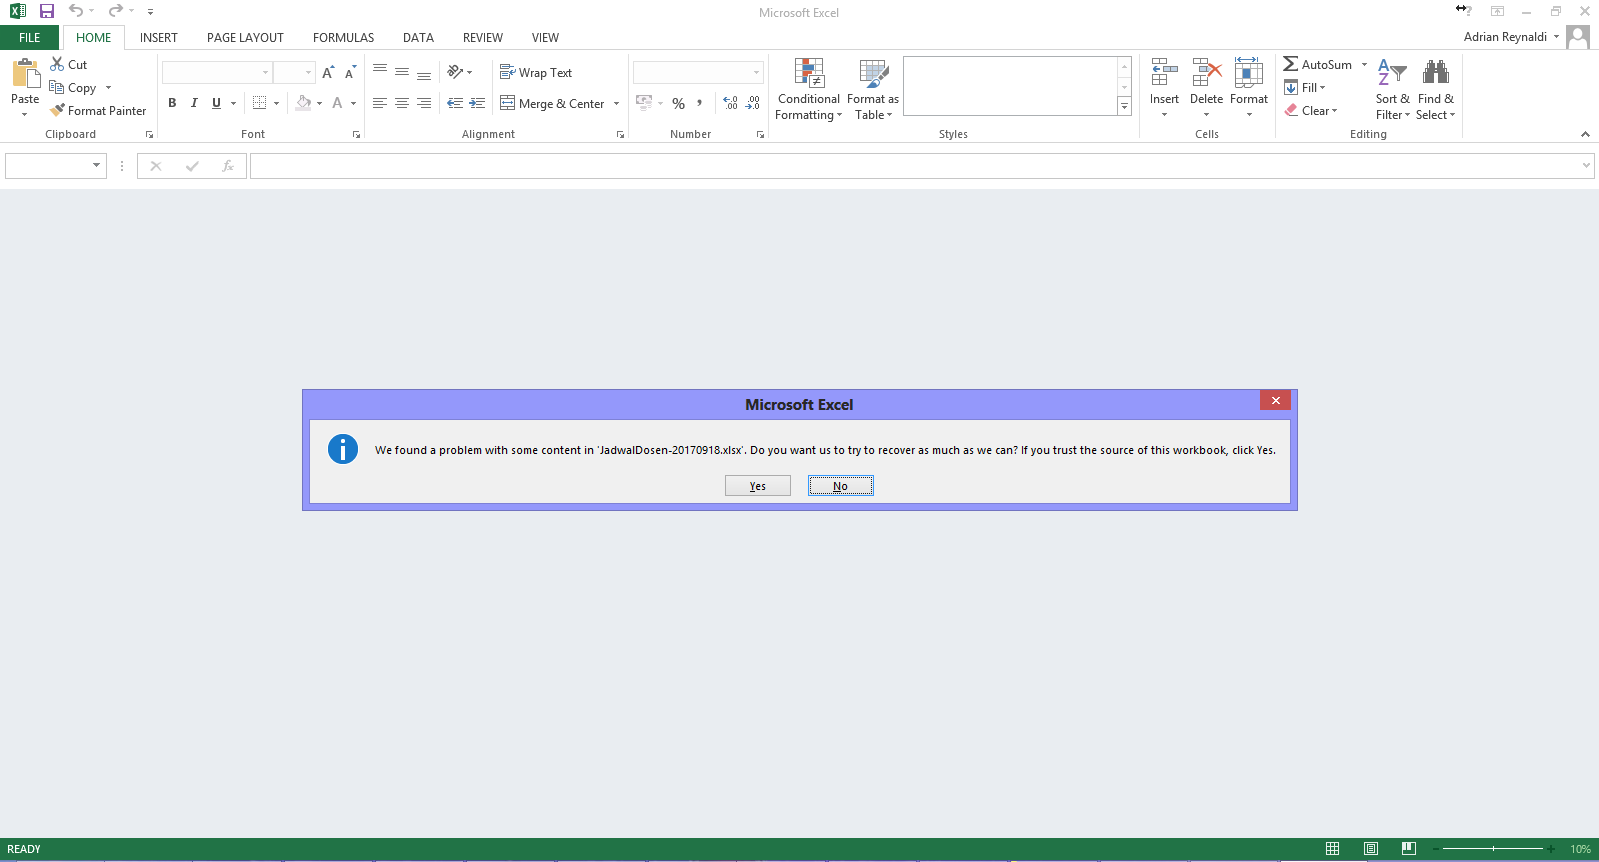
\includegraphics[scale=0.4]{erorXLSX.png}}
	\caption[Tampilan eror saat membuka file bertipe .xlsx]{Tampilan eror saat membuka file bertipe .xlsx} 
	\label{fig:flow-chart-CodeIgniter} 
\end{figure}

\begin{figure} [H]
	\centering  
	\frame{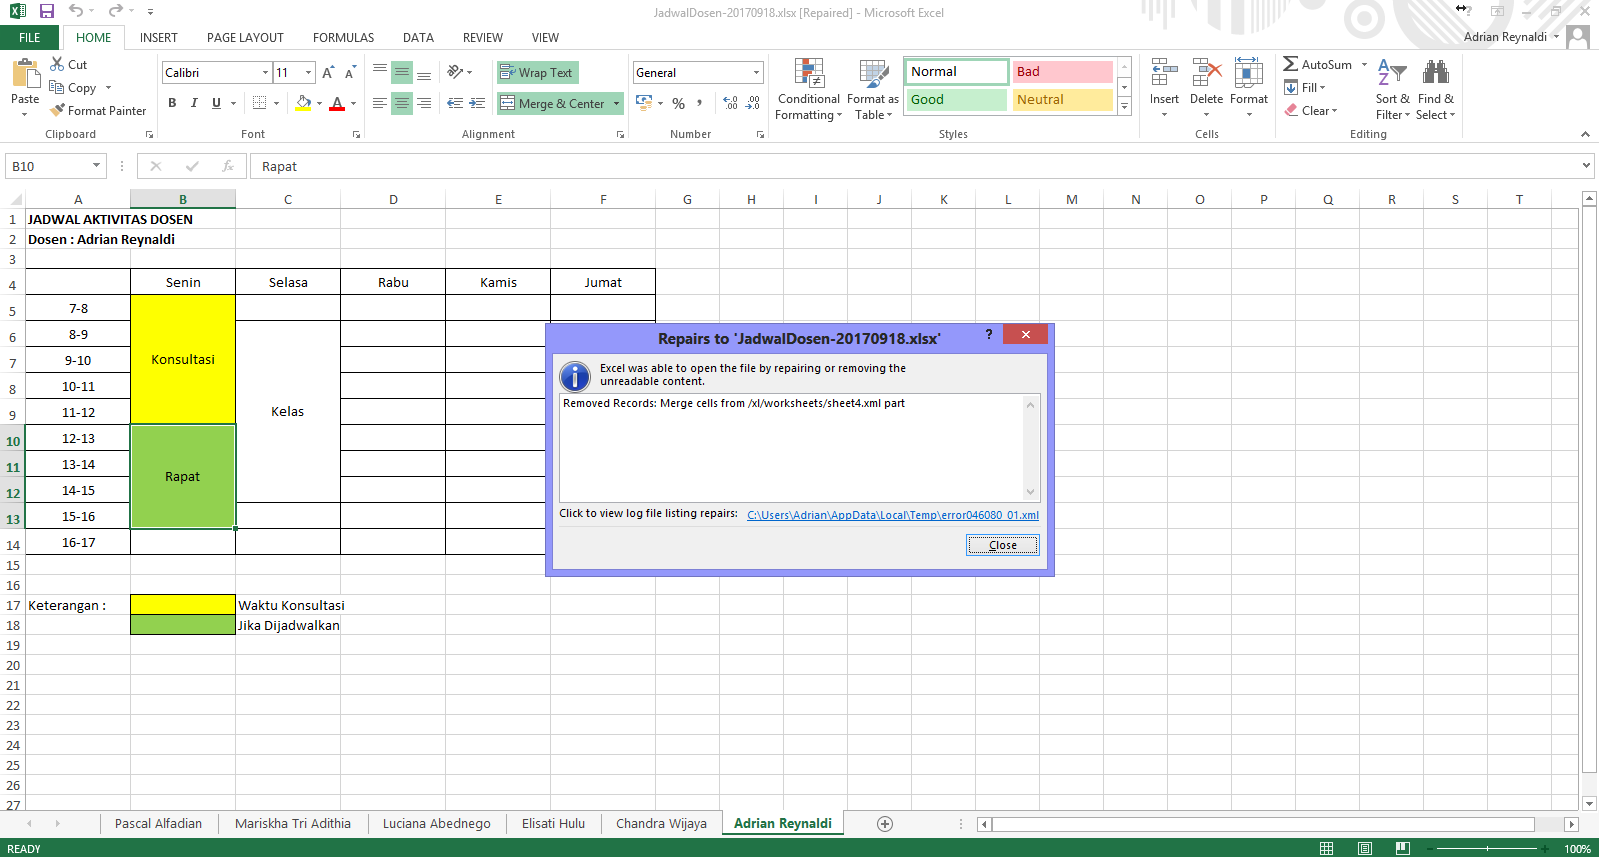
\includegraphics[scale=0.4]{erorXLSXDetail.png}}
	\caption[Keterangan Eror File .xlsx]{Keterangan Eror File .xlsx} 
	\label{fig:flow-chart-CodeIgniter} 
\end{figure}

Log eror:
\begin{lstlisting}
<?xml version="1.0" encoding="UTF-8" standalone="yes"?>
<recoveryLog xmlns="http://schemas.openxmlformats.org/spreadsheetml/2006/main">
<logFileName>error046080_01.xml</logFileName>
<summary>Errors were detected in file 'C:\Users\Adrian\Documents\Tugas\Skripsi\XLS Testing\JadwalDosen-20170918.xlsx'</summary>
<removedRecords summary="Following is a list of removed records:"><removedRecord>Removed Records: Merge cells from /xl/worksheets/sheet4.xml part
</removedRecord></removedRecords></recoveryLog>
\end{lstlisting}

\subsubsection{Hasil Pengujian dan Penyelesaian Masalah} 
\paragraph{}Dilihat dari log eror pada bagian Analisis di atas, eror terjadi karena ada perintah \textit{merge cells} yang dihapus oleh MS Excel. Hal ini terjadi karena adanya perintah dari PHPExcel versi 1.8.0 yang belum mendukung file bertipe .xlsx sehingga tab jadwal milik Ibu Mariskha tidak muncul. Maka karena eror disebabkan oleh permasalahan kompabilitas PHPExcel 1.8.0 dan tipe file .xlsx,  hal ini dapat diatasi dengan cara mengubah tipe file yang diekspor dari file .xlsx menjadi tipe yang lebih lama yaitu .xls.
\newline
\newline
Potongan kode lama yang menyebabkan eror:
\begin{lstlisting}[caption={Kode Lama},captionpos=b]
 $filename = 'JadwalDosen-'.date("Ymd").'.xlsx'; //Nama file XLS yang akan dibuat
 header('Content-type: application/vnd.ms-excel');
 header('Content-Disposition: attachment;filename="' . $filename . '"');

 $objWriter = PHPExcel_IOFactory::createWriter($this->excel, 'Excel2007');
\end{lstlisting}
Potongan kode baru untuk menghilangkan eror:
\begin{lstlisting}[caption={Kode Baru},captionpos=b]
 $filename = 'JadwalDosen-'.date("Ymd").'.xls'; //Nama file XLS yang akan dibuat
 header('Content-type: application/vnd.ms-excel');
 header('Content-Disposition: attachment;filename="' . $filename . '"');

 $objWriter = PHPExcel_IOFactory::createWriter($this->excel, 'Excel5');
\end{lstlisting}
Seperti bisa dilihat pada dua potongan kode program di atas, terjadi perubahan pada baris pertama kode dan baris terakhir kode. Pada baris pertama ekstensi file diubah dari .xlsx menjadi .xls. Pada baris terakhir tipe spreadsheet diubah dari 'Excel2007' menjadi 'Excel5'.
\paragraph{}Setelah tipe file diubah menjadi  .xls, eror di Microsoft Excel pun hilang.
\begin{figure} [H]
	\centering  
	\frame{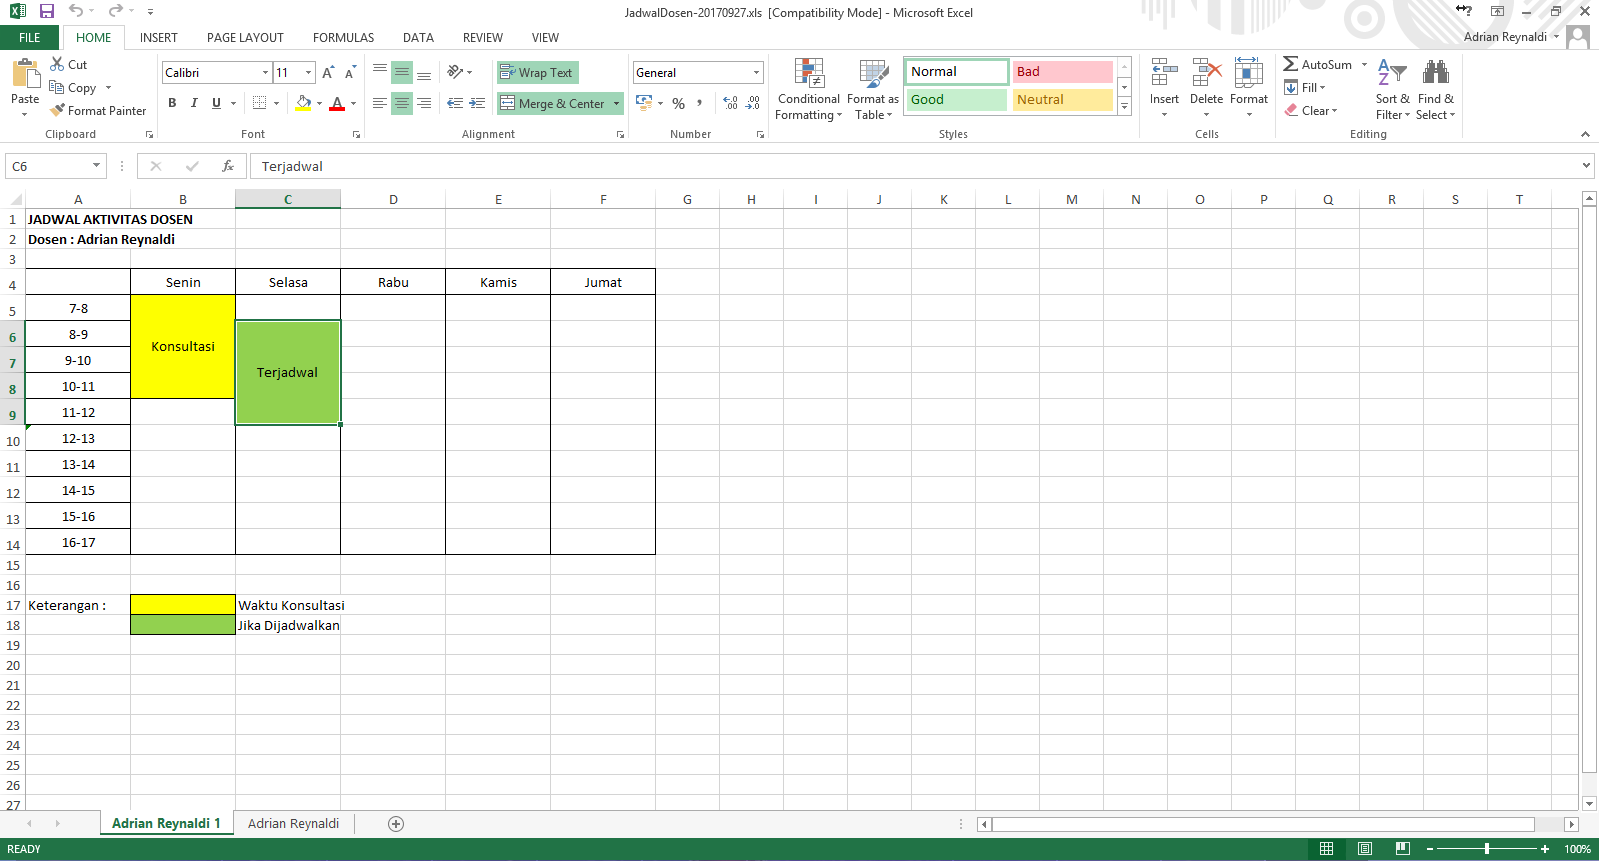
\includegraphics[scale=0.4]{tesXLSSukses.png}}
	\caption[Eror Sudah Tidak Muncul Ketika File Dibuka]{Eror Sudah Tidak Muncul Ketika File Dibuka} 
	\label{fig:eror-hilang} 
\end{figure}

\subsection{Pengujian Eksperimental Penambahan Tombol \textit{Delete All}}
\subsubsection{Masalah}
\paragraph{}Ketika jadwal yang dimasukan sudah sangat banyak, maka akan sulit untuk membersihkan tabel jadwal bila pengguna harus menghapus jadwal-jadwal tersebut satu per satu. Oleh karena itu Bapak Pascal mengusulkan untuk mengimplementasikan tombol "Delete All" yang berfungsi untuk menghapus semua jadwal yang sudah dimasukan oleh pengguna. 

\subsubsection{Analisis}
\paragraph{}Karena tombol "Delete All" ini memiliki pengaruh yang besar bila tidak sengaja tertekan oleh pengguna, maka diperlukan konfirmasi sebelum perintah penghapusan jadwal dieksekusi sistem.\newline
Untuk menangani itu diperlukan cara kerja sistem sebagai berikut:
\begin{enumerate}
	\item Ketika tombol "Delete All" ditekan akan ditampilkan \textit{pop-up} konfirmasi penghapusan jadwal.
	\item Lalu ketika tombol "ok" ditekan akan mengeksekusi perintah untuk menghapus semua jadwal milik user.
	\item Jika pengguna menekan tombol "cancel", sistem akan membatalkan perintah penghapusan jadwal dan menutup \textit{pop-up} konfirmasi.
\end{enumerate}
Untuk mengimplementasikan tombol "Delete All" diperlukan method tambahan pada controller EntriJadwalDosen dan JadwalDosen\_model untuk menghapus semua jadwal berdasarkan username/email pengguna..
\begin{center}
\begin{table}[H]
\caption{Perancangan method deleteAll di Controller EntriJadwalDosen}
\begin{tabular}{|c|p{11cm}|}
\hline
Nama Method 	& 	deleteAll 	\\
\hline
Parameter Input & email via POST \\
\hline
Parameter Output & - \\
\hline
Tabel yang berhubungan & jadwal\_dosen \\
\hline
Deskripsi	& Proses untuk memanggil method pada model JadwalDosen\_model untuk menghapus semua jadwal milik pengguna \\
\hline
Algoritma	& \begin{itemize}
				\item proses menerima input berupa email pengguna.
				\item proses memanggil method deleteByUsername(email) dari kelas JadwalDosen\_model dengan parameter email diisi dengan nama email pengguna.
				\end{itemize} \\
\hline
\end{tabular}
\end{table}
\end{center}

\begin{center}
\begin{table}[H]
\caption{Perancangan method deleteByUsername di Model JadwalDosen\_model}
\begin{tabular}{|c|p{11cm}|}
\hline
Nama Method 	& 	deleteByUsername 	\\
\hline
Parameter Input & email via POST \\
\hline
Parameter Output & - \\
\hline
Tabel yang berhubungan & jadwal\_dosen \\
\hline
Deskripsi	& Proses untuk menghapus semua jadwal milik pengguna di basis data\\
\hline
Algoritma	& \begin{itemize}
				\item proses menerima input berupa email dari controller EntriJadwalDosen.
				\item proses menghapus semua jadwal pengguna dari database.
				\end{itemize} \\
\hline
\end{tabular}
\end{table}
\end{center}

\subsubsection{Hasil Pengujian dan Penyelesaian Masalah}
Tombol "Delete All" dibuat di halaman EntriJadwalDosen di pojok kiri bawah.
\begin{figure} [H]
	\centering  
	\frame{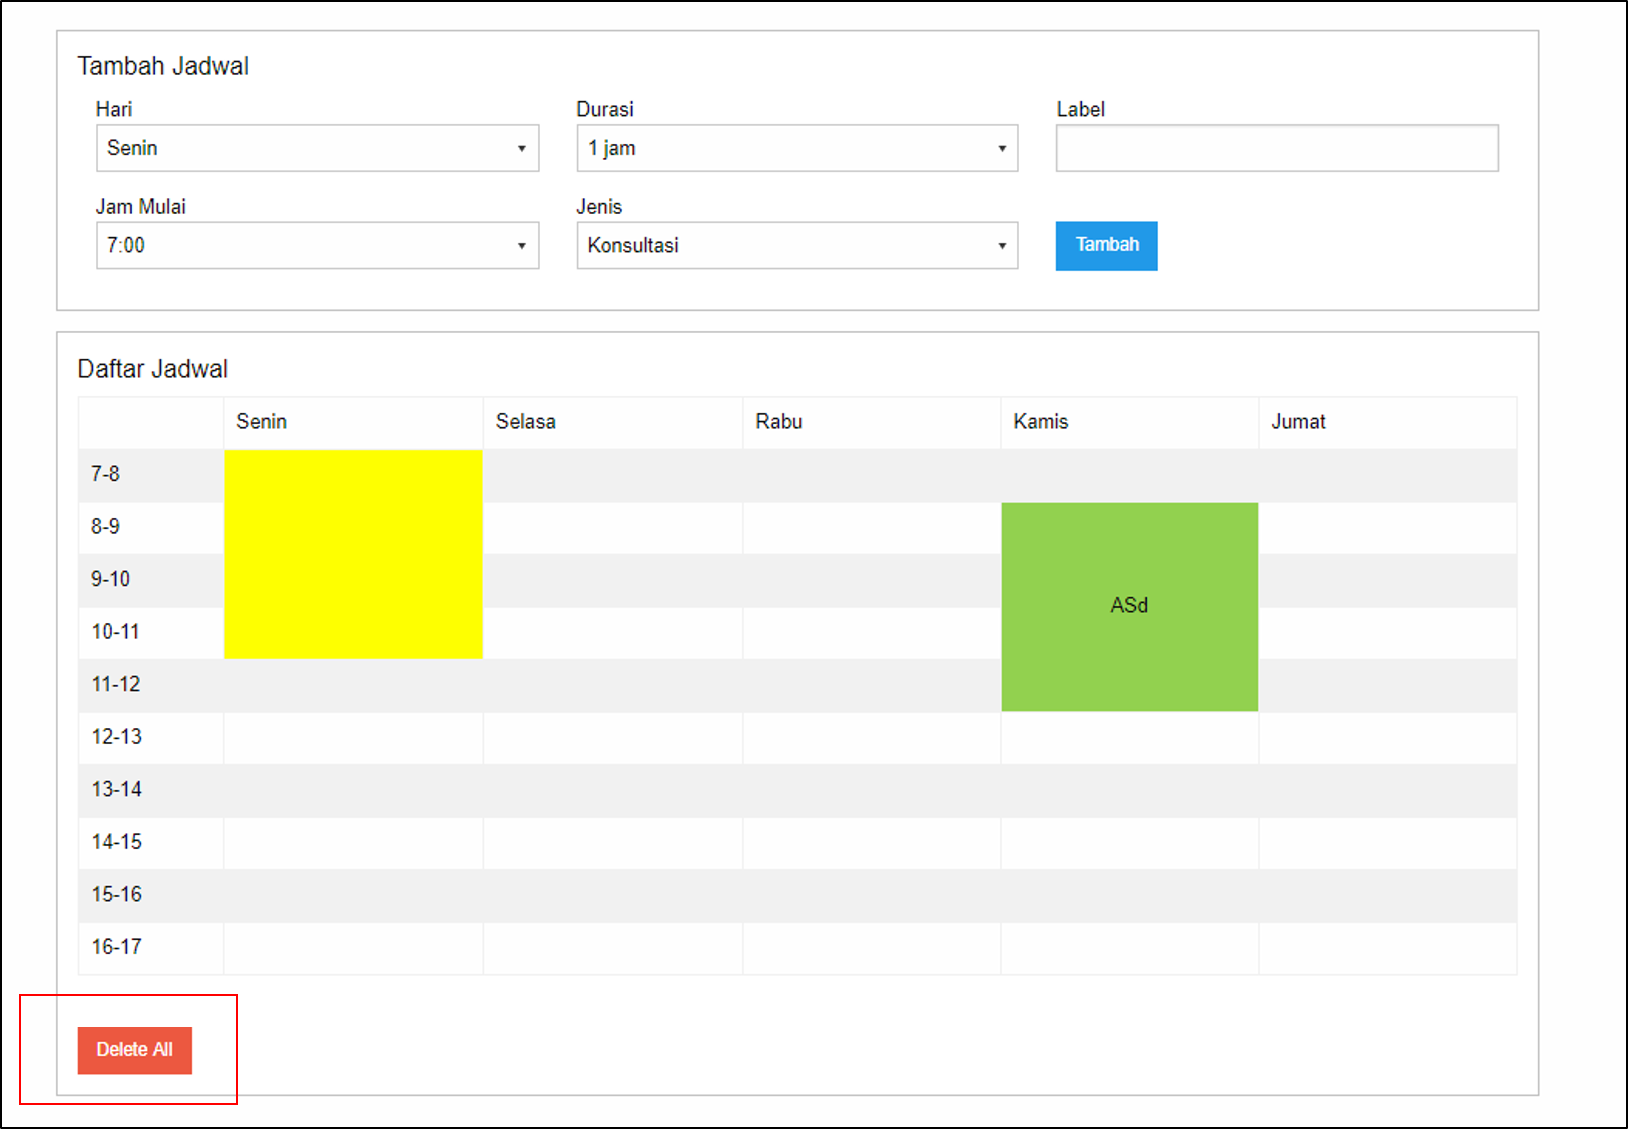
\includegraphics[scale=0.5]{deleteAllButton.png}}
	\caption[Tombol \textit{Delete All} di Entri Jadwal Dosen]{Tombol \textit{Delete All} di Entri Jadwal Dosen} 
\end{figure}
Ketika tombol "Delete All" ditekan memunculkan tampilan konfirmasi
\begin{figure} [H]
	\centering  
	\frame{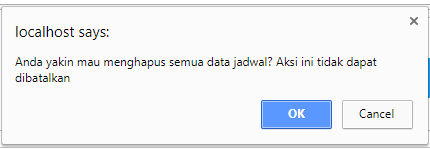
\includegraphics[scale=0.5]{popupDeleteAll.png}}
	\caption[Tampilan Konfirmasi]{Tampilan Konfirmasi} 
\end{figure}
Setelah tombol "ok" ditekan, semua jadwal dihapus
\begin{figure} [H]
	\centering  
	\frame{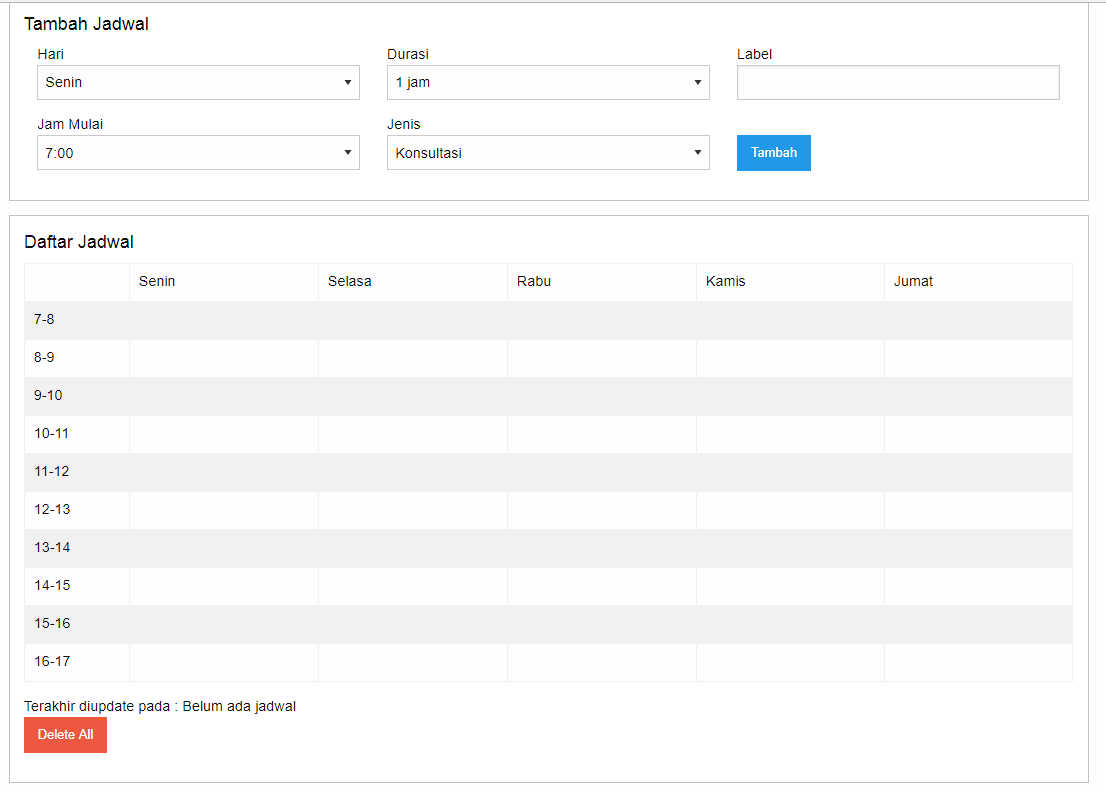
\includegraphics[scale=0.5]{empty.png}}
	\caption[Semua Jadwal Terhapus]{Semua Jadwal Terhapus} 
\end{figure}
Hasil pengujian berjalan lancar dan sesuai dengan hasil yang diharapkan.

\subsection{Pengujian Eksperimental Penambahan Informasi Waktu \textit{Update} Terakhir Jadwal}
\subsubsection{Masalah}
\paragraph{}Fitur ini merupakan usulan dari Bapak Pascal karena sering kali pengguna lupa kapan terakhir kali pengguna memasukan atau mengubah jadwal. Hal ini menyulitkan pengguna untuk mengetahui apakah jadwal yang telah ia masukan dapat dipakai atau tidak.
\subsubsection{Analisis}
\paragraph{}Informasi waktu \textit{update} terakhir jadwal oleh pengguna berfungsi agar pengguna dapat membedakan apakah jadwal miliknya merupakan versi lama yang sudah tidak dipakai atau merupakan versi baru. Hasil yang diharapkan adalah muncul label di halaman EntriJadwalDosen dan LihatJadwalDosen.\\
Untuk mengimplementasikan fitur ini perlu ditambahkan field baru di tabel jadwal\_dosen:
\begin{center}
\begin{table}[h]
\caption{Perancangan field tambahan di jadwal\_dosen}
\begin{tabular}{|c|c|c|c|c|c|}
 			\hline
		\textbf{Atribut} & \textbf{Tipe Data} & \textbf{Ukuran} & \textbf{PK* / FK*}  & \textbf{Keterangan} \\
			\hline
		 lastUpdate & datetime & - & bukan PK/FK &  tanggal terakhir jadwal di-\textit{update}\\
		 \hline
	\end{tabular}
	\end{table}
\end{center}
\subsubsection{Hasil Pengujian dan Penyelesaian Masalah}
Label yang bertuliskan informasi mengenai tanggal terakhir \textit{update} jadwal muncul di halaman EntriJadwalDosen
\begin{figure} [H]
	\centering  
	\frame{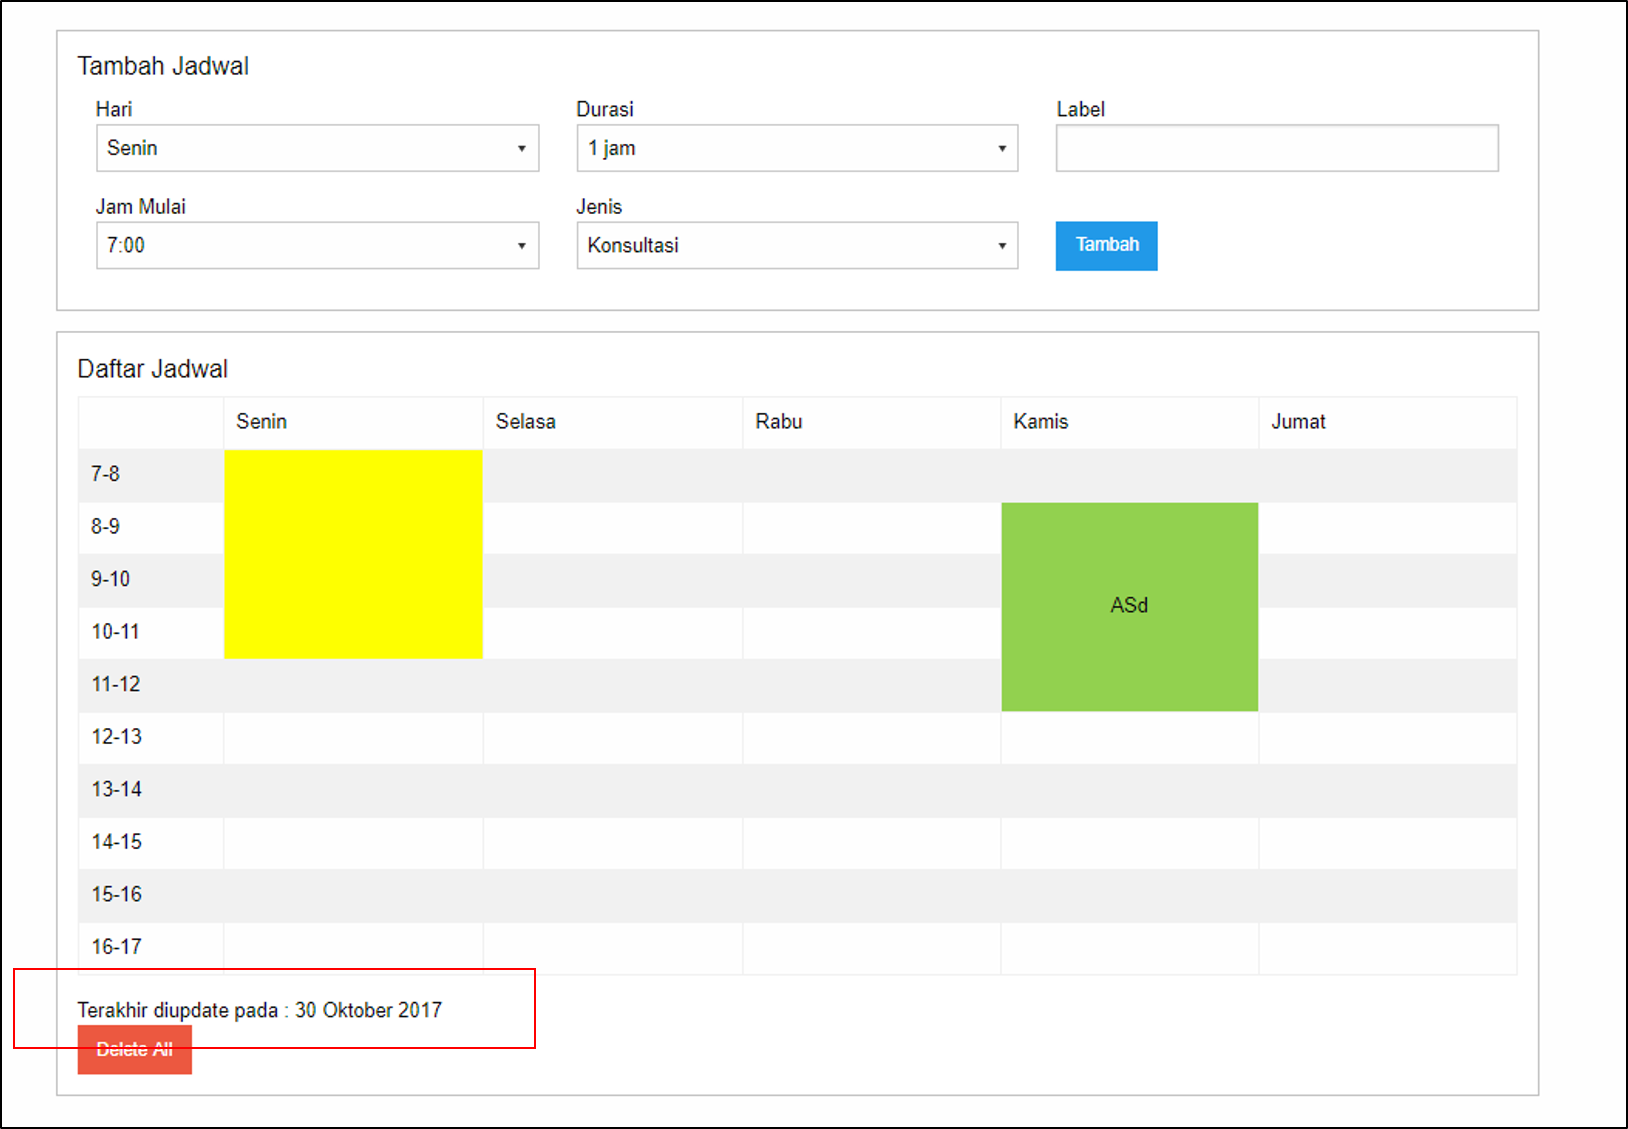
\includegraphics[scale=0.5]{updateTerakhir.png}}
	\caption[Informasi Waktu \textit{Update} Terakhir Jadwal di Entri Jadwal Dosen]{Informasi Waktu \textit{Update} Terakhir Jadwal di Entri Jadwal Dosen}
\end{figure}
Label berisi tanggal terakhir update jadwal muncul di halaman LihatJadwalDosen
\begin{figure} [H]
	\centering  
	\frame{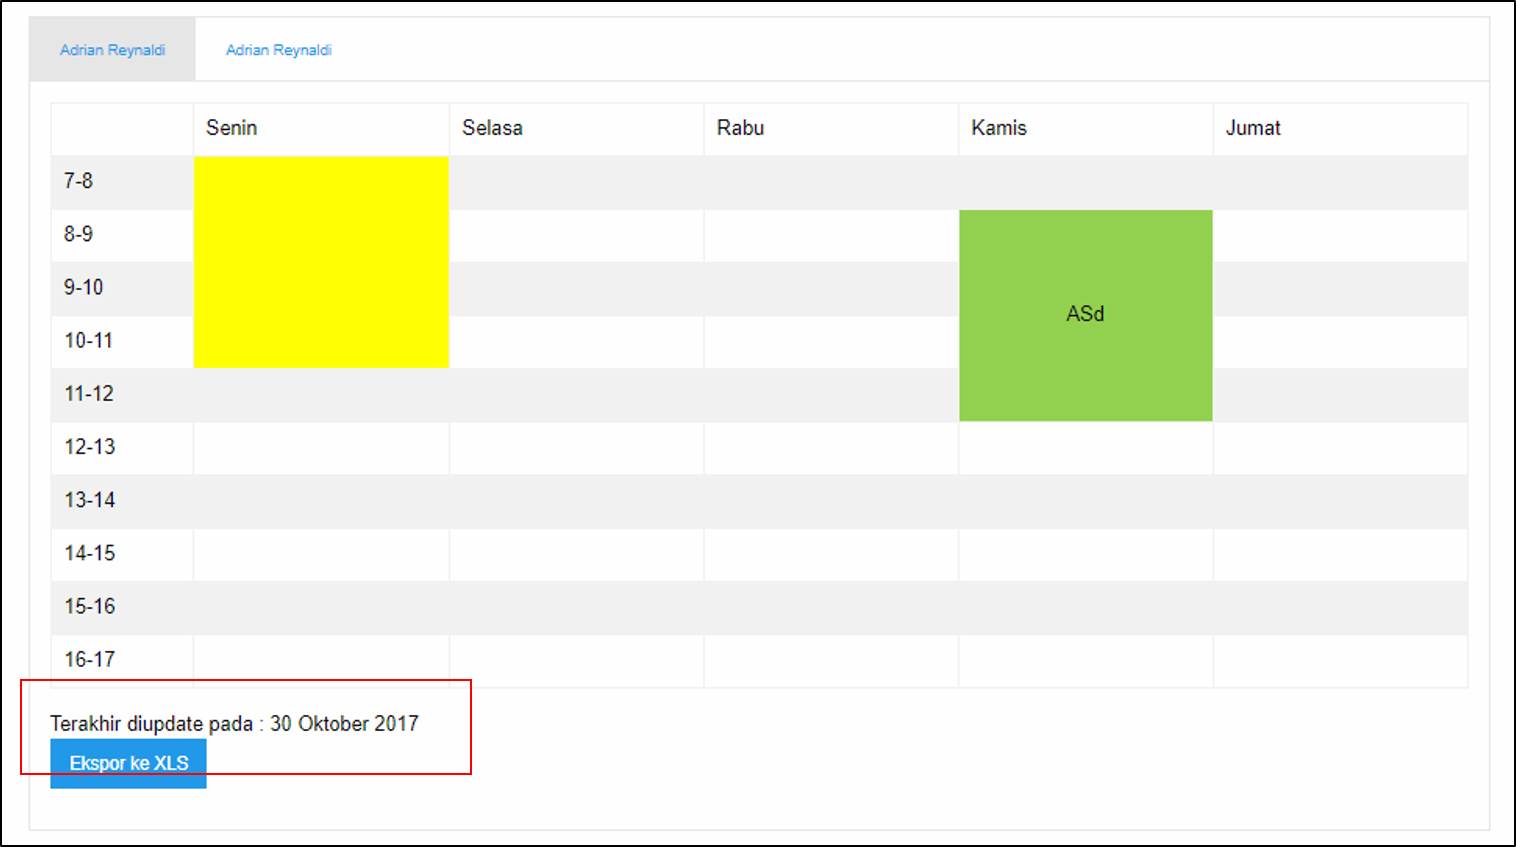
\includegraphics[scale=0.5]{updateTerakhirLihat.png}}
	\caption[Informasi Waktu \textit{Update} Terakhir Jadwal di Lihat Jadwal Dosen]{Informasi Waktu \textit{Update} Terakhir Jadwal di Lihat Jadwal Dosen}
\end{figure}
Hasil pengujian berjalan lancar dan sesuai dengan hasil yang diharapkan.

\subsection{Pengujian Eksperimental \textit{Conflict Handler}}
Conflict handler adalah fitur untuk menangani bentroknya jadwal.
\subsubsection{Masalah}
\paragraph{}Terdapat masalah bila ketika pengguna memasukan atau mengupdate jadwal, sistem tidak memeriksa apakah sudah ada jadwal pada waktu yang dimasukan oleh pengguna. Masalah ini merupakan masalah yang ditemukan oleh penulis sendiri.
\subsubsection{Analisis}
Untuk mencegah pengguna memasukan jadwal yang akan menimbulkan konflik dengan jadwal yang sudah ada, maka sistem perlu memeriksa:
\begin{itemize}
	\item Memeriksa apakah sudah ada jadwal di jam mulai jadwal baru.
	\item Memeriksa apakah sudah ada jadwal di jam akhir jadwal baru.
\end{itemize}
Untuk mencegah pengguna juga kebingungan ketika sistem menolak memasukan jadwal karena terjadinya konflik, maka perlu adanya:
\begin{itemize}
	\item Tampilan eror bahwa jadwal baru gagal dimasukan karena terjadi bentrok dengan jadwal lama.
	\item Tampilan eror bahwa edit jadwal gagal dilakukan karena terjadi bentrok dengan jadwal lain.
\end{itemize}
\subsubsection{Hasil Pengujian dan Penyelesaian Masalah}
Terdapat dua pengujian, yaitu pengujian pertama untuk memeriksa apakah konflik ketika memasukan jadwal baru sudah tertangani. Lalu pengujian kedua untuk memeriksa apakah konflik ketika mengubah jadwal yang menyebabkan bentrok dengan jadwal lain sudah ditangani.
\begin{enumerate}
	\item \textbf{Pengujian Pertama}\\
	Mencoba memasukan jadwal di hari Selasa jam 7 pagi ketika sudah ada jadwal lain di jam dan hari tersebut.
\begin{figure} [H]
	\centering  
	\frame{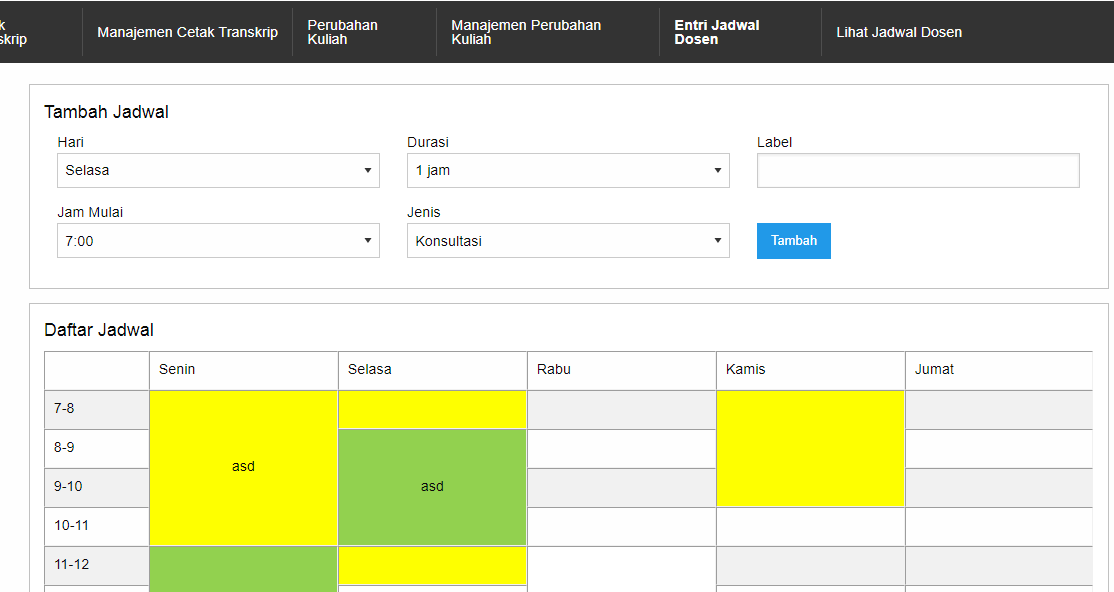
\includegraphics[scale=0.5]{memasukanBentrok.png}}
	\caption[Memasukan Jadwal ke Waktu yang Sudah Ada Jadwal]{Memasukan Jadwal ke Waktu yang Sudah Ada Jadwal} 
\end{figure}
	Muncul tampilan eror yang memberi tahu pengguna bahwa jadwal yang ingin dimasukan gagal masuk karena terjadi bentrok.
\begin{figure} [H]
	\centering  
	\frame{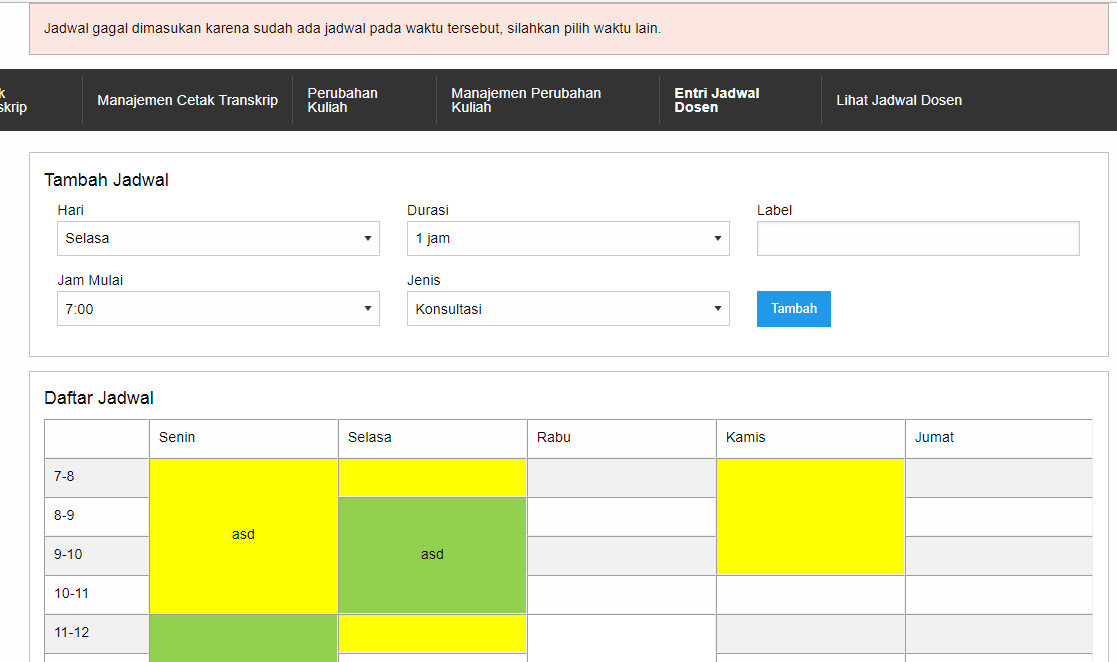
\includegraphics[scale=0.5]{GagalMasuk.png}}
	\caption[Tampilan Eror Gagal Masuk]{Tampilan Eror Gagal Masuk} 
\end{figure}

	\item \textbf{Pengujian Kedua}\\
	Daftar jadwal yang sudah ada dapat dilihat di Gambar 5.11
	\begin{figure} [H]
	\centering  
	\frame{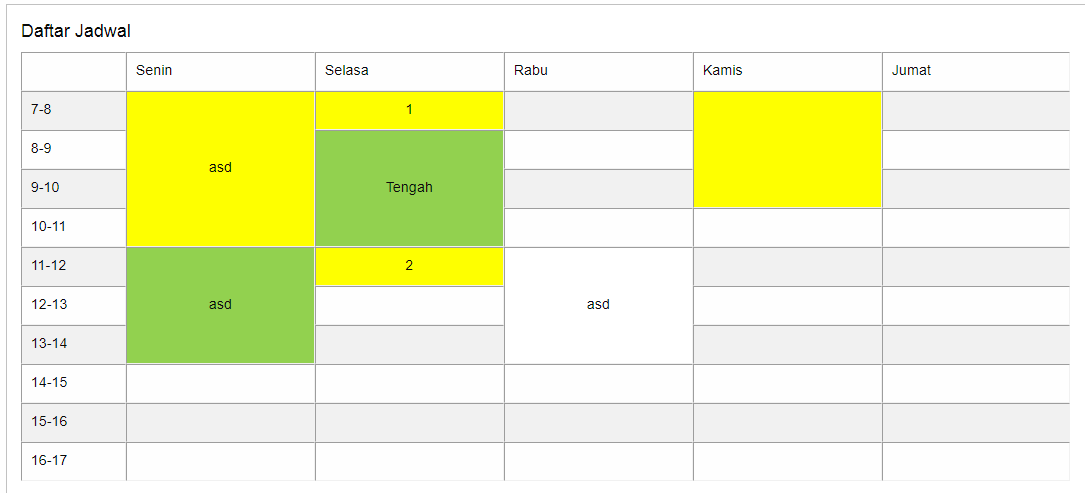
\includegraphics[scale=0.5]{daftarJadwal.png}}
	\caption[Jadwal yang Sudah Ada]{Jadwal yang Sudah Ada} 
	\end{figure}
	Mencoba mengubah jadwal "1" menjadi berdurasi 3 jam sehingga memicu bentrok dengan jadwal "Tengah".
	\begin{figure} [H]
	\centering  
	\frame{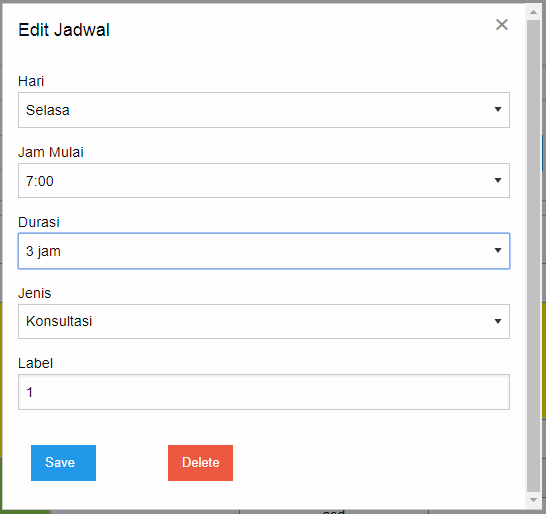
\includegraphics[scale=0.5]{mengeditBentrok.png}}
	\caption[Mengubah Jadwal "1"]{Mengubah Jadwal "1"} 
	\end{figure}
	Muncul tampilan eror yang memberi tahu bahwa jadwal gagal diubah.
	\begin{figure} [H]
	\centering  
	\frame{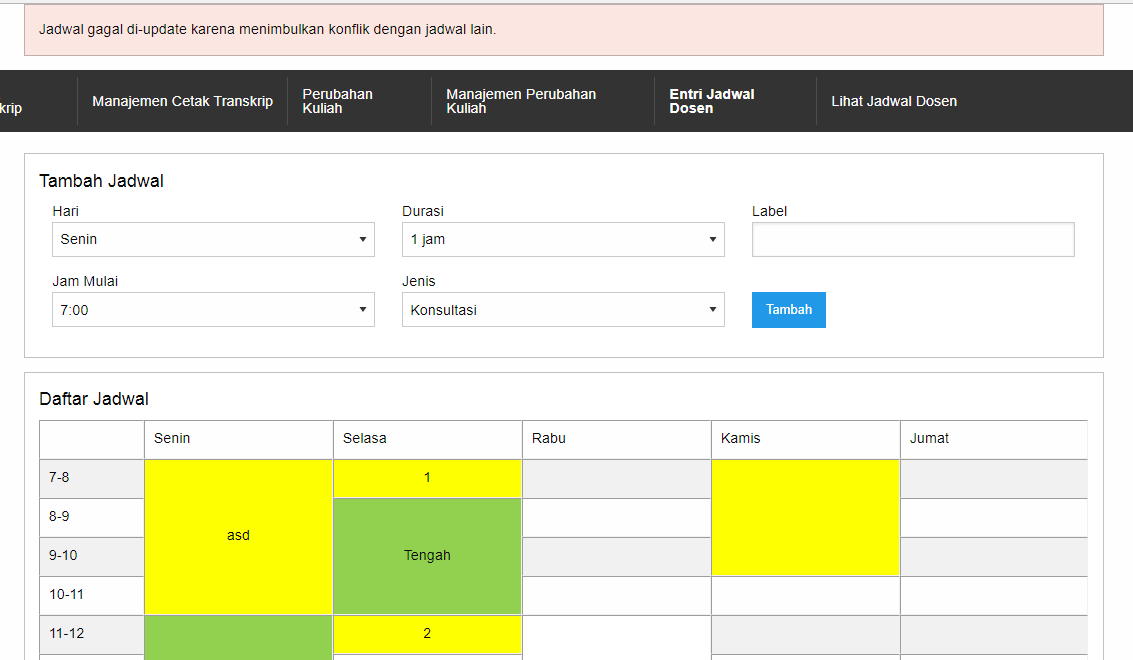
\includegraphics[scale=0.5]{gagalUpdate.png}}
	\caption[Tampilan Eror Gagal \textit{Update}]{Tampilan Eror Gagal \textit{Update}} 
	\end{figure}
	Mencoba mengubah jadwal "2" menjadi mulai pada jam 10 sehingga memicu bentrok dengan jadwal "Tengah".
	\begin{figure} [H]
	\centering  
	\frame{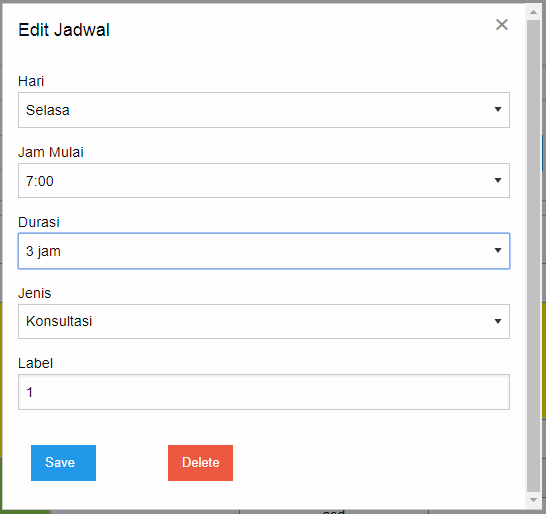
\includegraphics[scale=0.5]{mengeditBentrok.png}}
	\caption[Mengubah Jadwal "2"]{Mengubah Jadwal "2"} 
	\end{figure}
	Muncul tampilan eror yang memberi tahu bahwa jadwal gagal diubah.
	\begin{figure} [H]
	\centering  
	\frame{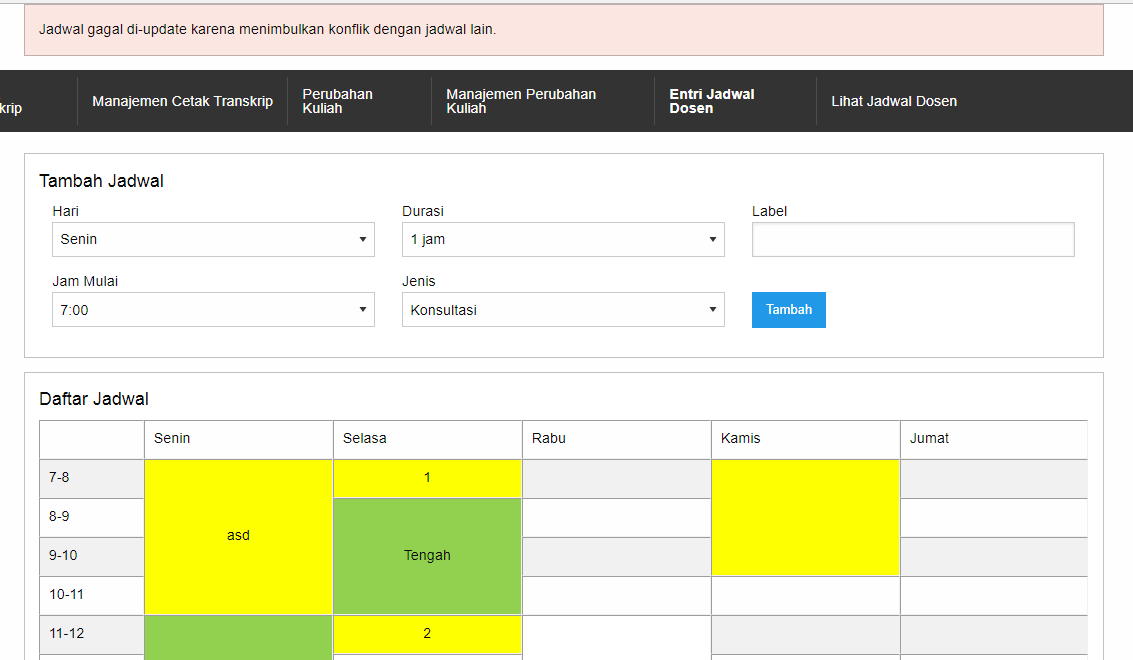
\includegraphics[scale=0.5]{gagalUpdate.png}}
	\caption[Tampilan Eror Gagal \textit{Update}]{Tampilan Eror Gagal \textit{Update}} 
	\end{figure}
\end{enumerate}
Setelah kedua pengujian di atas maka dapat disimpulkan pengujian berjalan dengan lancar dan hasil yang diharapkan tercapai.

\subsection{Pengujian Pada Browser Chrome, Firefox dan Internet Explorer}
Seringkali suatu website bekerja dalam satu browser, namun tidak bekerja pada browser lain. Oleh karena itu, pengujian ini digunakan untuk memastikan bahwa sistem bekerja pada 3 browser terpopuler yaitu Chrome, Firefox dan Internet Explorer.\footnote{https://www.w3schools.com/browsers/}
\subsubsection{Pengujian di Chrome}
Pengujian dilakukan menggunakan browser Google Chrome versi 63.0.3239.84 (32-bit). Berikut adalah hasil dari pengujian :
\begin{figure} [H]
	\centering  
	\frame{\includegraphics[scale=0.5]{Chrome1.png}}
	\caption[Pengujian Menu Login]{Pengujian Menu Login} 
	\end{figure}
\begin{figure} [H]
	\centering  
	\frame{\includegraphics[scale=0.5]{Chrome2.png}}
	\caption[Pengujian Modul EntriJadwalDosen]{Pengujian Modul EntriJadwalDosen} 
	\end{figure}
\begin{figure} [H]
	\centering  
	\frame{\includegraphics[scale=0.5]{Chrome2.png}}
	\caption[Pengujian Modul LihatJadwalDosen]{Pengujian Modul LihatJadwalDosen} 
	\end{figure}
Semua modul berhasil dijalankan pada browser ini.
\subsubsection{Pengujian di Firefox}
Pengujian dilakukan menggunakan Firefox Quantum versi 57.0.2 (64-bit).
\begin{figure} [H]
	\centering  
	\frame{\includegraphics[scale=0.5]{Firefox1.png}}
	\caption[Pengujian Menu Login]{Pengujian Menu Login} 
	\end{figure}
\begin{figure} [H]
	\centering  
	\frame{\includegraphics[scale=0.5]{Firefox2.png}}
	\caption[Pengujian Modul EntriJadwalDosen]{Pengujian Modul EntriJadwalDosen} 
	\end{figure}
\begin{figure} [H]
	\centering  
	\frame{\includegraphics[scale=0.5]{Firefox3.png}}
	\caption[Pengujian Modul LihatJadwalDosen]{Pengujian Modul LihatJadwalDosen} 
	\end{figure}
Semua modul berhasil dijalankan pada browser ini.

\subsubsection{Pengujian di Internet Explorer}
Pengujian dilakukan menggunakan Internet Explorer 10 yang dirilis pada tahun 2013.
\begin{figure} [H]
	\centering  
	\frame{\includegraphics[scale=0.5]{IE1.png}}
	\caption[Pengujian Menu Login]{Pengujian Menu Login} 
	\end{figure}
\begin{figure} [H]
	\centering  
	\frame{\includegraphics[scale=0.5]{IE2.png}}
	\caption[Pengujian Modul EntriJadwalDosen]{Pengujian Modul EntriJadwalDosen} 
	\end{figure}
\begin{figure} [H]
	\centering  
	\frame{\includegraphics[scale=0.5]{IE3.png}}
	\caption[Pengujian Modul LihatJadwalDosen]{Pengujian Modul LihatJadwalDosen} 
	\end{figure}
Semua modul berhasil dijalankan pada browser ini.
\subsubsection{Kesimpulan Pengujian Pada Browser Berbeda}
Semua modul sistem Aplikasi Perekam Jadwal Dosen berhasil dijalankan di ketiga browser Chrome, Firefox dan Internet Explorer. Berdasarkan statistik pengguna browser yang didapat dari \textit{https://www.w3schools.com/browsers/} dapat diprediksi 93.6\% pengguna internet dapat mengakses sistem  tanpa masalah.
\subsection{Kesimpulan Pengujian Eksperimental}
\paragraph{}Semua pengujian eksperimental berhasil, meskipun pada awal setiap pengujian sistem memiliki banyak kendala teknis seperti misalnya kompabilitas PHPExcel dengan program Microsoft Excel itu sendiri. Masalah-masalah tersebu berhasil ditangani dengan mempelajari lebih dalam setiap bagian-bagian sistemnya dan melakukan modifikasi pada kode-kode sistem. Dengan demikian sistem sudah berhasil diimplementasikan ke dalam BlueTape dan siap digunakan untuk para pengguna.